\documentclass{beamer}
\usetheme{Warsaw}
\usepackage{hyperref}
\usepackage{amsmath}
\newcommand{\argmax}{\operatornamewithlimits{argmax}}
\usefonttheme[onlymath]{serif}

\title{Clockwork RNN - ICML14}
\author{Seungwoo Yoo}
\date{\today}

\begin{document}
\begin{frame}
  \vspace*{1.5cm}\titlepage  
  \centering Many figures are from Alex Graves phD thesis. 
\end{frame}

\section[Outline]{}
\frame{\tableofcontents}

\section{Introduction}
\frame
{
	\frametitle{About the authors}
    \begin{figure}[ht]  
		\begin{center}
			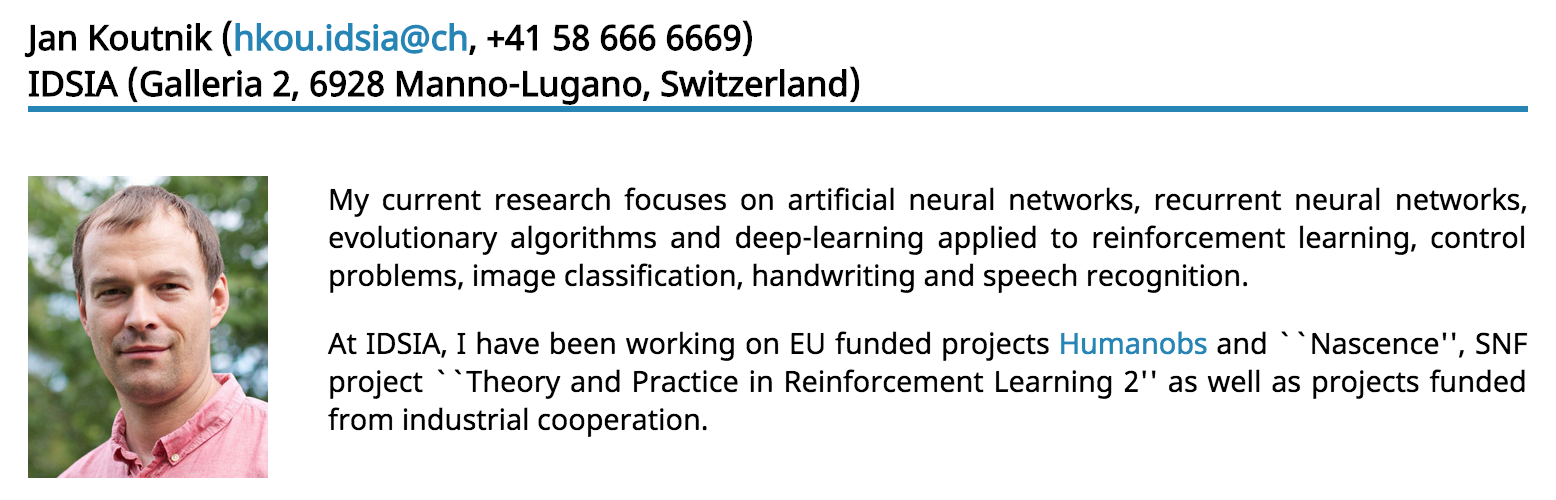
\includegraphics[width=4.1in]{Images/author.png}   
		\end{center}   
		\caption{Main author - Jan Koutnik}
	\end{figure}
}
\frame
{
	\frametitle{Contributions}
	\begin{itemize}
        \item Introduce a new RNN structure \textit{Clockwork} RNN (CW-RNN) :
			\begin{enumerate}
			\item Hidden layer is partitioned into separate module
			\item Each processing inputs at its own clock rate
			\end{enumerate}
		\item Contribution points
			\begin{itemize}
			\item CW-RNN reduces the number of RNN parameters
			\item Improve the performance and speed up the network evaluation
            \item Esp., audio signal generation and TIMIT spoken word classification
			\end{itemize}
	\end{itemize}
}
\section{Brief summary to RNN/LSTM}
\frame
{
    \frametitle{RNN summary - Forward pass}
    \begin{columns}[c]
    		\column{.3\textwidth}
		\begin{figure}[ht]  
			\begin{center}
				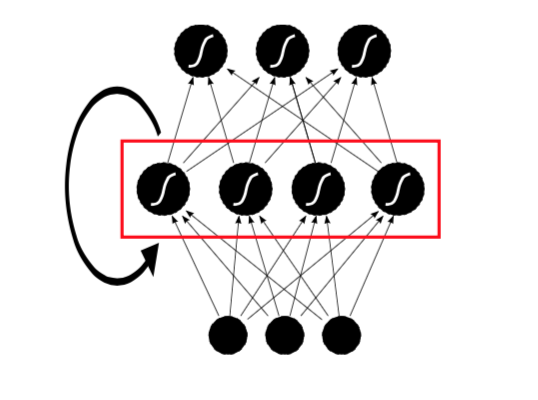
\includegraphics[width=1.6in]{Images/recurrentNN.png}   
			\end{center}   
		\end{figure}
    		\column{.6\textwidth}
			\begin{figure}[ht]  
    			\begin{center}
    				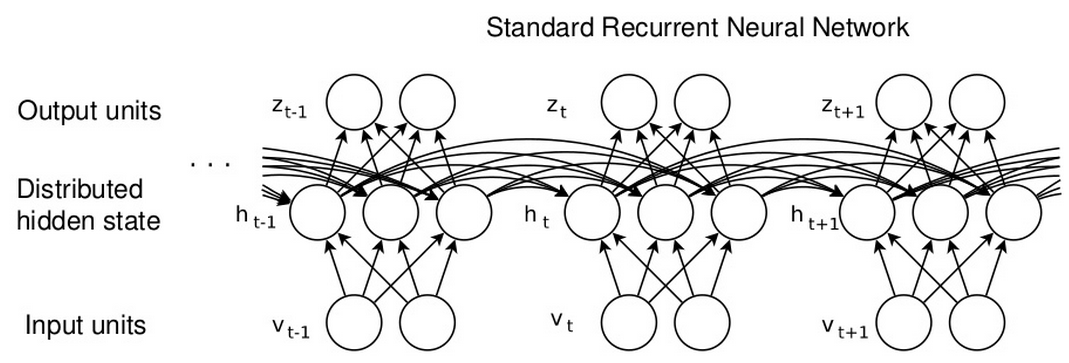
\includegraphics[width=2.6in]{Images/standard_rnn.png}       			
    			\end{center}
    			\end{figure}
	\end{columns}
    \begin{itemize}
        \item Hidden units : 
        $ a_h^t = {\sum_{i=1}^I} W_{ih}x_i^t + \sum_{h'=1}^H w_{h'h} {b_{h'}}^{t-1} $ \\
        Usually initial values $b_i^0$ are chosen to zero / 
        Some cases RNN stability can be improved by using nonzero initial values.
        \item Actifaction function :
        $ b_h^t = \theta_h(a_h^t) $
        \item Output units : 
        $ a_k^t = \sum_{h=1}^H w_{hk}b_h^t $
    \end{itemize}
}
\frame
{
    \frametitle{RNN summary - Backward pass \\ Backpropagation through time (BPTT)}
    \begin{itemize}
        \item Like standard backpropagtion, consists of a repeated chain rule (depends on the next $t+1$ state) \\ 
            \vspace{0.1in}
            $ \delta_h^t = \theta'(a_h^t) \Big( \sum_{k=1}^K \delta_k^t w_{hk} + 
            \sum_{h'=1}^H \delta_{h'}^{t+1} w_{hh'} \Big)$ \\
            \vspace{0.1in}
            where $\delta_j^t \equiv \frac{\partial O}{\partial a_j^t} $
        \item Since the weights to and from each unit in the hidden layer are the same at every time step, 
            we need to sum over the whole sequence to get the derivatives : \\
            \vspace{0.1in}
            $ \frac{\partial O}{\partial w_{ij}} = \sum_{t=1}^T \frac{\partial O}{\partial a_j^t} \frac{\partial a_j^t}{\partial w_{ij}} = \sum_{t=1}^T \delta_j^t b_i^t $
    \end{itemize}
}
\frame
{
    \frametitle{BDRNN summary}
	\begin{figure}[ht]  
		\begin{center}
			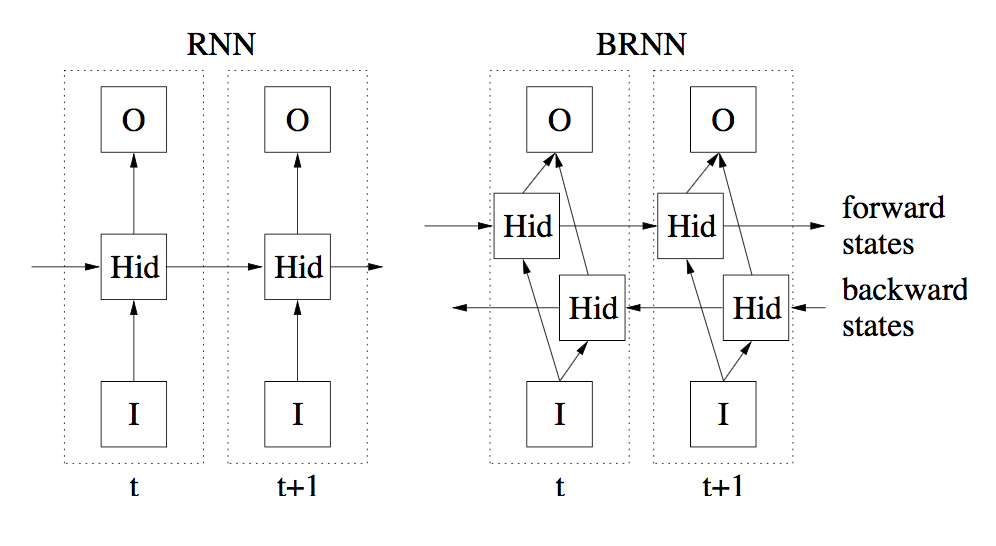
\includegraphics[width=2.2in]{Images/BDRNN_RNN.png}   
		\end{center}   
		\caption{Comparison between BDRNN and RNN}
	\end{figure}
    \begin{itemize}
        \item BDRNN (Bidirectional recurrent neural network) 
        \item Present each training sequence forwards and backwards to two seperate recurrent hidden layers, 
            both of which are connected to the same output layer
    \end{itemize}
}
\frame
{
    \begin{itemize}
        \item Forward pass for BDRNN 
            \begin{itemize} 
                \item Generally same as for a undirectional RNN, 
                \item The input sequence is presented in opposite directions to the two hidden layers. 
                \item The ouput layer is not updated until both hidden layers have processed the entire input sequence:
	            \begin{figure}[ht]  
	            	\begin{center}
	            		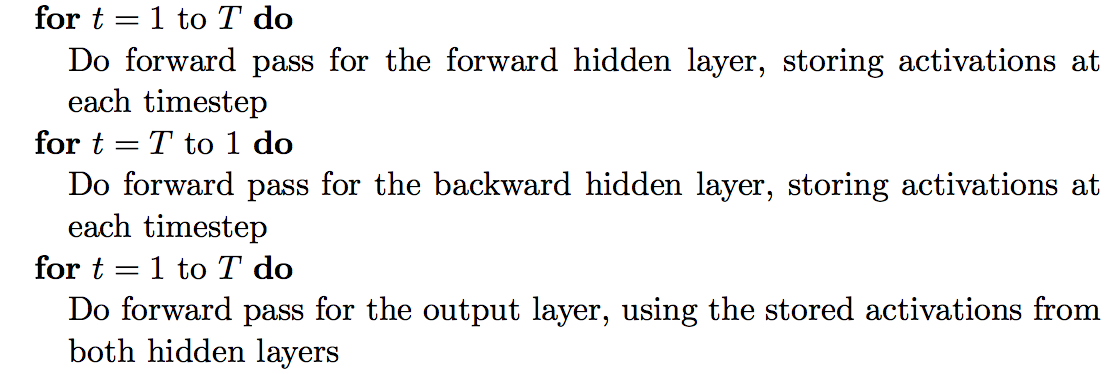
\includegraphics[width=3.5in]{Images/BDRNN_forward_pass.png}   
	            	\end{center}   
	            \end{figure}
            \end{itemize}
    \end{itemize}
}
\frame
{
    \begin{itemize}
        \item Backward pass for BDRNN 
            \begin{itemize} 
                \item Similar to the backward pass proceeds as for a standard RNN training with BPTT  
                \item All the output layer $ \delta $ terms are calculated first, 
                    then fed back to the two hidden layers in opposite directions:
	            \begin{figure}[ht]  
	            	\begin{center}
	            		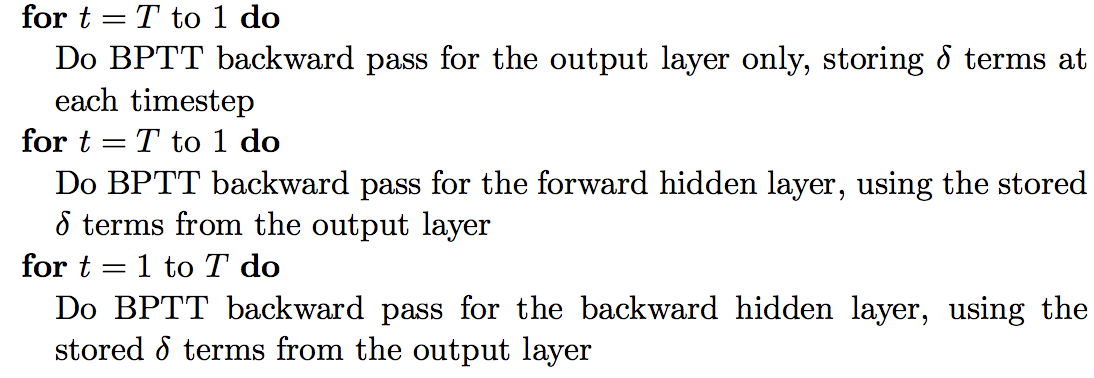
\includegraphics[width=3.5in]{Images/BDRNN_backward_pass.png}   
	            	\end{center}   
	            \end{figure}
            \end{itemize}
    \end{itemize}
}
\frame
{
    \begin{itemize}
        \item BDRNN and Causal tasks 
            \begin{itemize} 
                \item For tasks requiring future inputs, BDRNN cannot be applied (e.g., financial prediction, robot navigation and etc.)  
                \item A task where the input sequences are spatial and not temporal is rightly applicable (e.g., protein prediction)
                \item However, some temporal tasks can also be applied, as long as the network outputs are only needed at the end of some input segment (e.g., speech and handwriting recognition - data is usually divided up into sentences, lines, or dialogue turns and etc.)
            \end{itemize}
    \end{itemize}
}
\frame
{
    \frametitle{LSTM summary}
	\begin{figure}[ht]  
		\begin{center}
			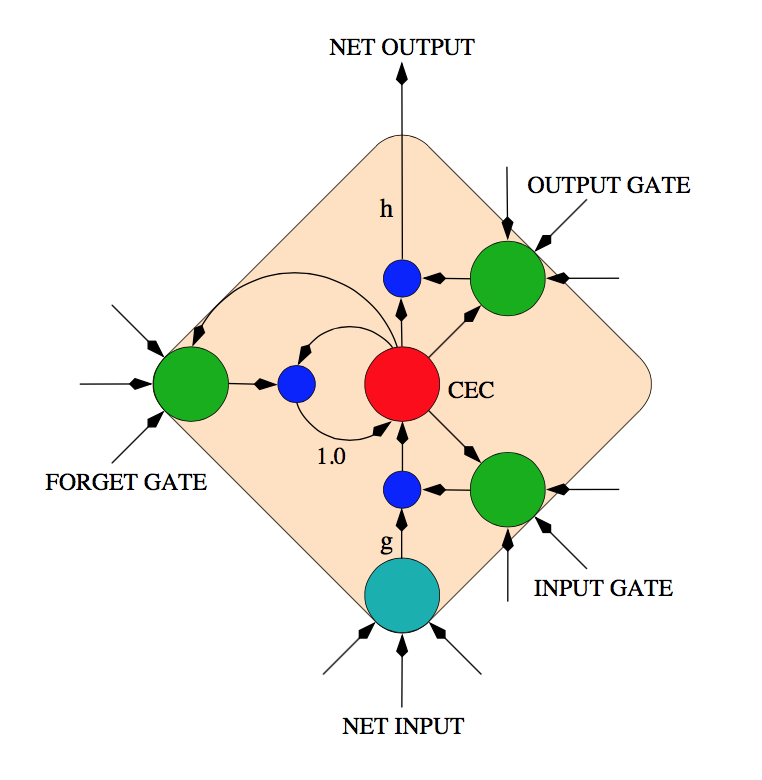
\includegraphics[width=2.2in]{Images/LSTM.png}   
		\end{center}   
		\caption{LSTM structure}
	\end{figure}
}
\frame
{
	\begin{figure}[ht]  
		\begin{center}
			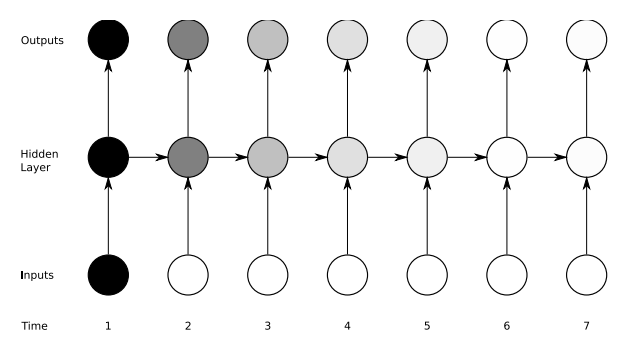
\includegraphics[width=3.2in]{Images/rnn_vanishing_gradients.png}   
		\end{center}   
		\caption{Vanishing gradient problem for RNNs}
	\end{figure}
	\vspace{-0.5cm}
	\begin{itemize}
		\item The sensitivity of the network decays exponentially over time as new inputs overwrite the activation of hidden unit and the network "forgets" the first input. 
	\end{itemize}
}
\frame
{
	\begin{columns}
		\column{0.5\textwidth}
		\begin{figure}[ht]  
			\begin{center}
				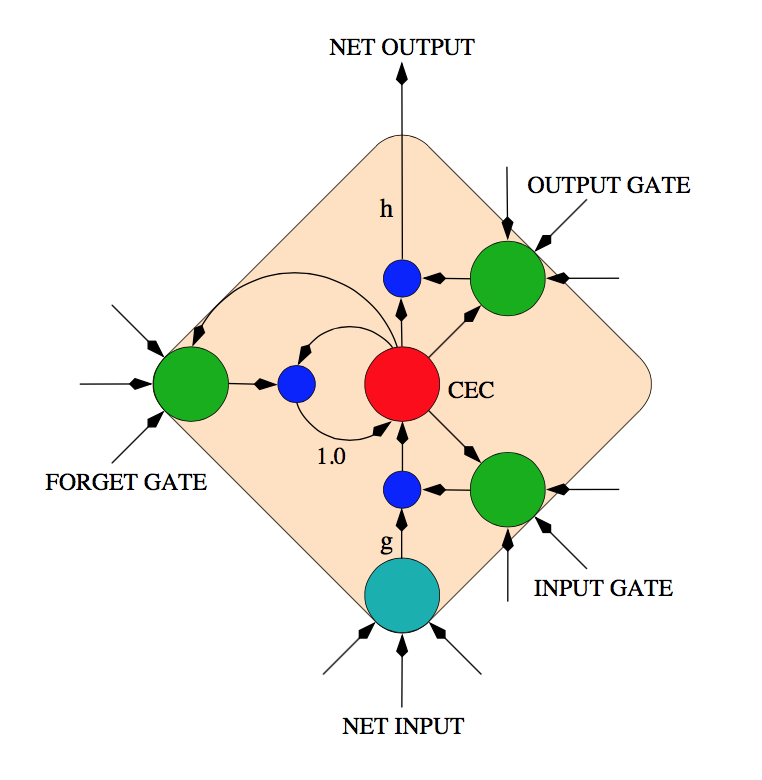
\includegraphics[width=2.1in]{Images/LSTM.png}   
			\end{center}   
			\caption{\centering LSTM memory block with a single cell}
		\end{figure}
		\column{0.6\textwidth} 
		\begin{itemize}
		\item LSTM architecture - consists of a set of memory blocks	
		\item Each block contains one or multiple self-connected memory cells and three multiplicative units	(analogous to memory chips in digital computer)
			\begin{enumerate}
			\item the input gate - write
			\item the output gate - read
			\item the forget gate - reset
			\end{enumerate}
		\end{itemize}
	\end{columns}
}
\frame
{
	\begin{columns}
		\column{0.5\textwidth}
		\begin{figure}[ht]  
			\begin{center}
				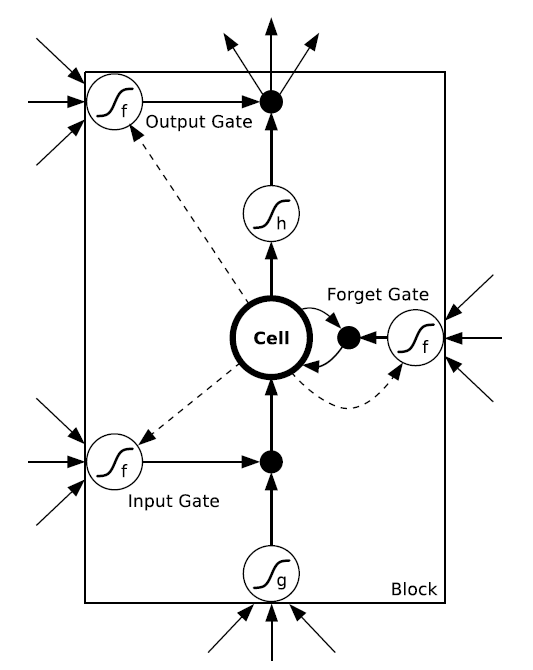
\includegraphics[width=1.8in]{Images/LSTM_detail.png}   
			\end{center}   
			\caption{\centering LSTM memory block with a single cell}
		\end{figure}
		\column{0.4\textwidth} 
		\begin{itemize}
		\item Input / output gates multiply the input and and ouput of the cell 
		\end{itemize}
	\end{columns}
}
\frame
{
		\begin{figure}[ht]  
			\begin{center}
				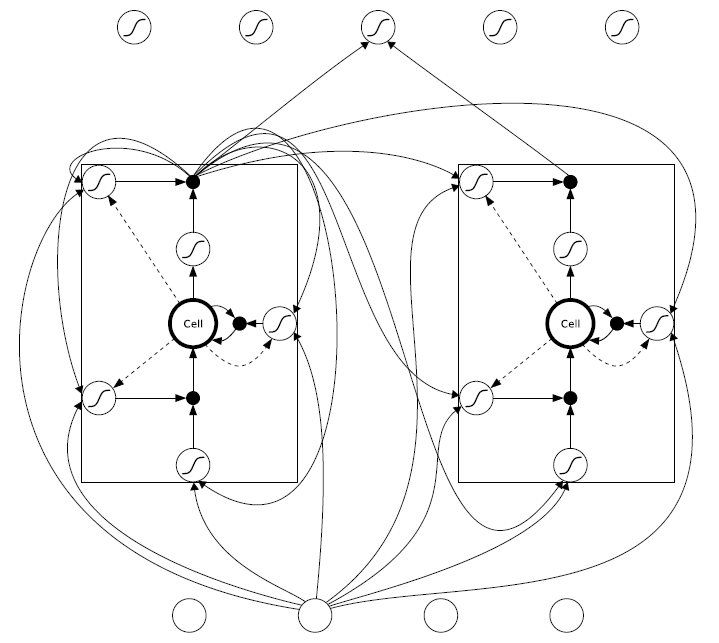
\includegraphics[width=2.6in]{Images/LSTM_network.png}   
			\end{center}   
			\caption{\centering LSTM network consisting of four input units / a hidden layer of two single-cell LSTM memory blocks and five output units}
		\end{figure}
}
\frame
{
		\begin{figure}[ht]  
			\begin{center}
				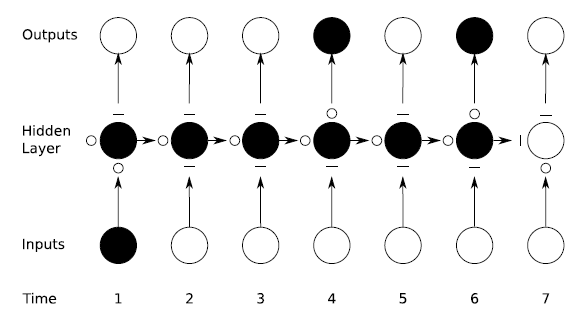
\includegraphics[width=2.6in]{Images/LSTM_preserving_gradient.png}   
			\end{center}   
			\caption{\centering Preservation of gradient information by LSTM}
		\end{figure}
}
\frame
{
  \frametitle{Some comments from Andrew Ng}
   \begin{figure}[ht]  
		\begin{center}
			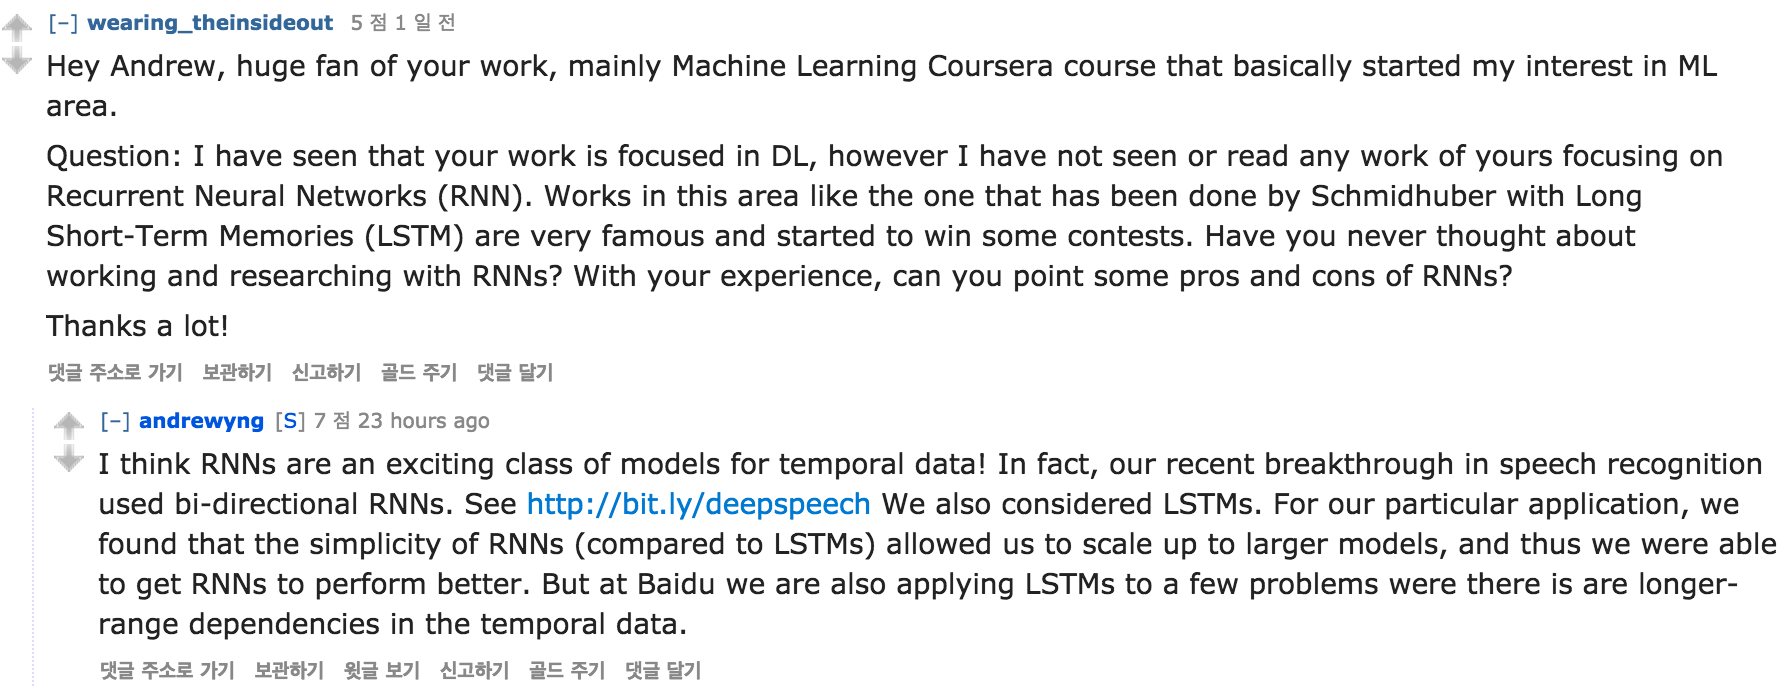
\includegraphics[width=4.5in]{Images/comment_rnn_ng.png}   
		\end{center}   
		\caption{Comments from Andrew Ng of RNN}
	\end{figure}
}
\section{Clockwork RNN (CwRNN)}
\frame
{
   \frametitle{Some comments from Schmidhuber}
   \begin{figure}[ht]  
		\begin{center}
			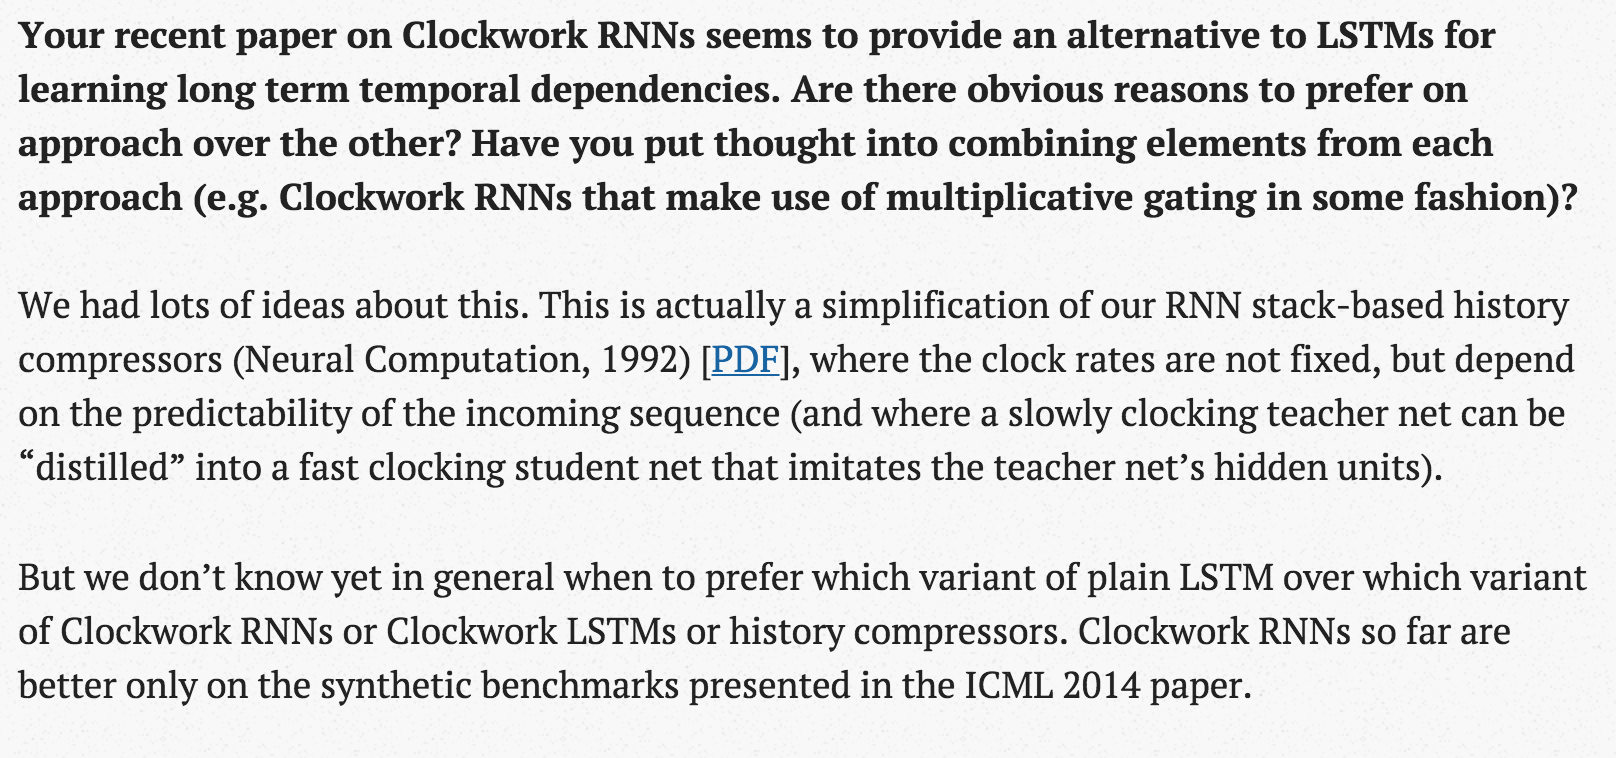
\includegraphics[width=4.2in]{Images/comment_cwrnn.png}   
		\end{center}   
		\caption{Comments from Schmidhuber of Clockwork RNN}
	\end{figure}
}
\end{document}
